\documentclass[tikz,border=6pt]{standalone}
\usetikzlibrary{arrows.meta}
\begin{document}
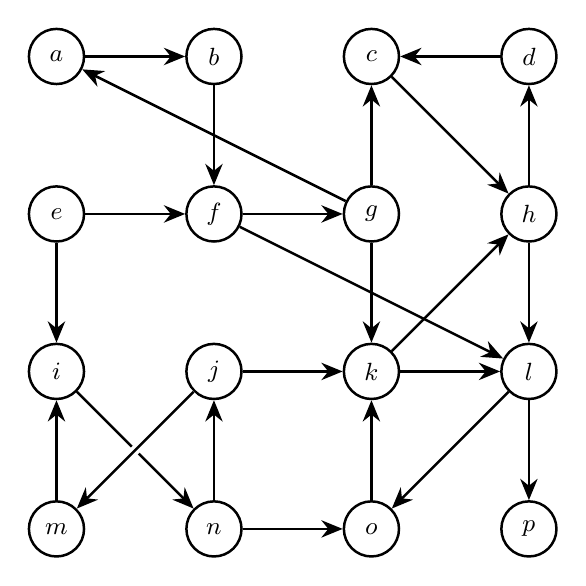
\begin{tikzpicture}[
  vertex/.style={circle,draw=black,line width=0.9pt,fill=white,
    minimum size=7mm,inner sep=0pt,font=\small},
  edge/.style={-{Stealth[length=2.7mm,width=2.2mm]},draw=black,line width=0.9pt},
  x=2cm,y=2cm
]
% Labels run left to right, then top to bottom.
\foreach \name/\x/\y in {
  a/0/3,b/1/3,c/2/3,d/3/3,
  e/0/2,f/1/2,g/2/2,h/3/2,
  i/0/1,j/1/1,k/2/1,l/3/1,
  m/0/0,n/1/0,o/2/0,p/3/0}
  \node[vertex] (\name) at (\x,\y) {$\name$};
% Every original graph edge is retained, with a uniform appearance.
\foreach \from/\to in {
  a/b,b/f,g/a,g/c,c/h,d/c,h/d,
  e/f,e/i,f/g,f/l,g/k,h/l,
  i/n,j/k,k/h,k/l,l/o,l/p,
  m/i,n/j,n/o,o/k}
  \draw[edge] (\from) -- (\to);
% A small white underlay distinguishes the crossing diagonals.
\draw[edge,preaction={draw=white,line width=3.5pt,-}] (j) -- (m);
\end{tikzpicture}
\end{document}
